\subsection{Túnel de vento}

%SLIDE DE TUNEL DE VENTO
%\begin{frame}
%\frametitle{Túnel de vento}
%
%Os túneis de vento são estruturas que propiciam a simulação para o desenvolvimento de estudos que relacionam o efeito do movimento de ar em torno de objetos, como turbinas, aviões, carros e edificações. 
%
%\begin{itemize}
%    \item Circuito: Aberto e fechado.
%    \item Vel. escoamento: Subsônico, supersônico e hipersônico.
%    \item Para aberto: Soprador e sugador.
%\end{itemize}
%
%\end{frame}

%SLIDE DE TUNEL DE VENTO
\begin{frame}
\frametitle{Túnel de vento}

O túnel de vento tratado neste trabalho está situado junto ao Laboratório de Sistemas Térmicos da Universidade Federal do Rio Grande e é de característica subsônica, circuito aberto e do tipo soprador.

\begin{figure}
\centering
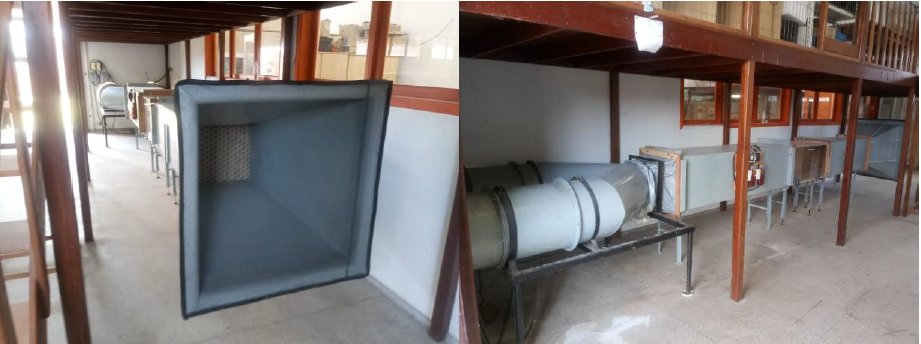
\includegraphics[scale = 0.4]{figuras/tunelfran}
\end{figure}

\end{frame}
